\documentclass[
	classe=$1^{ere}STI2D$
]{évaluation}

\usepackage{tikz-repère}
\usepackage{tcolorbox}

\begin{luacode}
function SUITE(init, rec)
	local f = function (n)
		local x = init
		while n ~= 0 do
			x = rec(x)
			n = n - 1
		end
		return x
	end
	return f
end
\end{luacode}

\date{7 avril 2023}

\begin{document}

\newcommand{\makeCorrection}{}
\title{Évaluation : suites (Sujet A)}
\maketitle

\begin{exercice}
	\begin{enumerate}[a)]
		\item Définie par récurrence, géométrique
		\item Définie par récurrence, arithmétique
		\item Définie explicitement, arithmétique
		\item Définie par récurrence, ni arithmétique ni géométrique
	\end{enumerate}
\end{exercice}

\begin{exercice}
	Soit $u$ la suite définie par $u₀ = 2$ et $u_{n+1} = 0,5uₙ + 5$.

	\begin{enumerate}
		\item
		      \begin{multicols}{4}
			      \begin{itemize}
				      \item $u₁ = 6$
				      \item $u₂ = 8$
				      \item $u₃ = 9$
				      \item $u₄ = 9,5$
			      \end{itemize}
		      \end{multicols}

		      \begin{center}
			      \begin{tikzpicture}[scale=0.5]
				      \tikzRepere{0.5}{4}{0.5}{10}
				      \foreach \x/\y in {1/6,2/8,3/9,4/9.5} {
						      \node at (\x,\y) {×};
						      \node[below left] at (\x,\y) {$u_{\x}$};
					      }
			      \end{tikzpicture}
		      \end{center}
		\item $u$ semble être croissante.
		\item $u_2 - u_1 = 2$ et $u_3 - u_2 = 1$, donc $u$ n'est pas arithmétique. \medskip

		      $\dfrac{u_2}{u_1} = \dfrac{4}{3}$ et $\dfrac{u_3}{u_2} = \dfrac{9}{8}$, donc $u$ n'est pas géométrique.
		\item
		      \begin{multicols}{4}
			      \begin{itemize}
				      \item $v₀ = -8$
				      \item $v₁ = -4$
				      \item $v₂ = -2$
				      \item $v₃ = -1$
			      \end{itemize}
		      \end{multicols}
		\item $v$ semble être géométrique de raison $0,5$.
		\item \begin{align*}
			      \dfrac{v_{n+1}}{vₙ} & = \dfrac{u_{n+1} - 10}{uₙ - 10} \\
			                          & = \dfrac{0,5uₙ - 5}{uₙ - 10}    \\
			                          & = 0,5\dfrac{uₙ- 10}{uₙ - 10}    \\
			                          & = 0,5                           \\
		      \end{align*}

		      Donc $v$ est géométrique de raison $0,5$.
	\end{enumerate}
\end{exercice}

\begin{exercice}
	\begin{enumerate}
		\item Au bout d'une année, notre salaire devient $1200 × 1,08 - 20 = 1276$€. On a donc bien une augmentation de $76$€.
		\item \begin{itemize}
			      \item $a_1 = 1300$, et $a_{n+1} = a_n + 70$
			      \item $b_1 = 1200$, et $b_{n+1} = b_n × 1,08 - 20$
		      \end{itemize}
		\item
		      \correctionOr{
			      \begin{center}
				      \directlua{function SCALE(x) return x / 100 - 12 end}
				      \begin{tikzpicture}
					      \tikzRepere{0}{10}{0}{11}[][]
					      \foreach \y in {0,...,11} {
							      \pgfmathsetmacro\valy{int(1200 + 100*\y)}
							      \draw[thick] (0,\y) -- ++(-0.2,0) node[left] {$\valy$};
						      }
					      \foreach \x in {0,...,10} {
							      \draw[thick] (\x,0) -- ++(0,-0.2) node[below] {$\x$};
							      \pgfmathsetmacro\entrpA{(13 + 0.7*\x) - 12}
							      \node at (\x,\entrpA) {×};
							      \node at (\x,\directlua{tex.print(SCALE(SUITE(1200, function(x) return x * 1.08 - 20 end)(\x)))}) {×};
						      }
				      \end{tikzpicture}
			      \end{center}
		      }{}
		\item Il faut donc $5$ ans pour que le salaire de l'entreprise $B$ dépasse celui de l'entreprise $A$.
	\end{enumerate}
\end{exercice}

\begin{exercice}
	\begin{enumerate}
		\item La suite $v$ est arithmétique.
		\item \begin{multicols}{3}
			      \begin{itemize}
				      \item $v_1 = v_0 - 9,8 = -9,8$
				      \item $v_2 = v_1 - 9,8 = -19,6$
				      \item $v_3 = v_2 - 9,8 = -29,4$
			      \end{itemize}
		      \end{multicols}
		      $v$ est décroissante.
		\item On a $p(4) = -98$m, et $p(5) = -147$m. Le poids a donc touché le sol entre la quatrième et la cinquième seconde.
	\end{enumerate}
\end{exercice}

%======================================================
%===================== SUJET B ========================
%======================================================
\newpage
\setcounter{exercice}{1}

\title{Évaluation : suites (Sujet B)}
\maketitle

\begin{exercice}
	\begin{enumerate}[a)]
		\item Définie par récurrence, arithmétique
		\item Définie par récurrence, géométrique
		\item Définie par récurrence, ni arithmétique ni géométrique
		\item Définie explicitement, arithmétique
	\end{enumerate}
\end{exercice}

\begin{exercice}
	Soit $u$ la suite définie par $u₀ = 2$ et $u_{n+1} = 0,5uₙ + 13$.

	\begin{enumerate}
		\item \begin{multicols}{4}
			      \begin{itemize}
				      \item $u₁ = 14$
				      \item $u₂ = 20$
				      \item $u₃ = 23$
				      \item $u₄ = 24,5$
			      \end{itemize}
		      \end{multicols}

		      \begin{center}
			      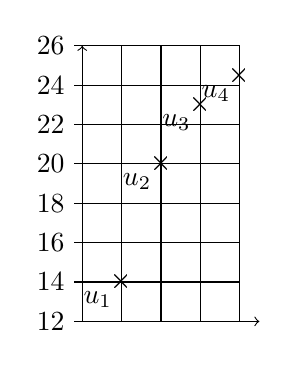
\begin{tikzpicture}[scale=0.5]
				      \draw (0,0) grid (4,7);
				      \draw[->] (0,0) -- ++(4.5,0);
				      \draw[->] (0,0) -- ++(0,7);
				      \foreach \y in {12,14,...,26} {
						      \draw (0,\y/2 - 6) -- ++(-0.2,0) node[left] {$\y$};
					      }

				      \foreach \x/\y in {1/1,2/4,3/5.5,4/6.25} {
						      \node at (\x,\y) {×};
						      \node[below left] at (\x,\y) {$u_{\x}$};
					      }
			      \end{tikzpicture}
		      \end{center}
		\item $u$ semble être croissante.
		\item $u_1 - u_0 = 12$, et $u_2 - u_1 = 7$, donc $u$ n'est pas arithmétique. \medskip

		      $\dfrac{u_1}{u_0} = 7$ et $\dfrac{u_2}{u_1} = \dfrac{10}{7} ≈ 1,43$, donc $u$ n'est pas géométrique.
		\item
		      \begin{multicols}{4}
			      \begin{itemize}
				      \item $v₀ = -24$
				      \item $v₁ = -12$
				      \item $v₂ = -6$
				      \item $v₃ = -3$
			      \end{itemize}
		      \end{multicols}
		\item $v$ semble être géométrique de raison $0,5$
		\item \begin{align*}
			      \dfrac{v_{n+1}}{vₙ} & = \dfrac{u_{n+1} - 26}{uₙ - 26} \\
			                          & = \dfrac{0,5uₙ - 13}{uₙ - 26}   \\
			                          & = 0,5\dfrac{uₙ- 26}{uₙ - 26}    \\
			                          & = 0,5                           \\
		      \end{align*}

		      Donc $v$ est géométrique de raison $0,5$.
	\end{enumerate}
\end{exercice}

\begin{exercice}
	\begin{enumerate}
		\item La première année, le salaire dans l'entreprise $B$ devient $1300 × 1,08 - 20 = 1384$€. On a donc bien une augmentation, de $84$€.
		\item \begin{itemize}
			      \item $a_0 = 1400$, $a_{n+1} = a_n + 70$
			      \item $b_0 = 1300$, $b_{n+1} = b_n × 1,08 - 20$
		      \end{itemize}
		\item \begin{center}
			      \directlua{function SCALE(x) return x / 100 - 13 end}
			      \begin{tikzpicture}
				      \tikzRepere{0}{10}{0}{12}[][]
				      \foreach \y in {0,...,12} {
						      \pgfmathsetmacro\valy{int(1300 + 100*\y)}
						      \draw[thick] (0,\y) -- ++(-0.2,0) node[left] {$\valy$};
					      }
				      \foreach \x in {0,...,10} {
						      \draw[thick] (\x,0) -- ++(0,-0.2) node[below] {$\x$};
						      \pgfmathsetmacro\entrpA{(14 + 0.7*\x) - 13}
						      \node at (\x,\entrpA) {×};
						      \node at (\x,\directlua{tex.print(SCALE(SUITE(1300, function(x) return x * 1.08 - 20 end)(\x)))}) {×};
					      }
			      \end{tikzpicture}
		      \end{center}
		\item Il faut donc $5$ ans pour que le salaire de l'entreprise $B$ dépasse celui de l'entreprise $A$.
	\end{enumerate}
\end{exercice}

\begin{exercice}
	\begin{enumerate}
		\item La suite $v$ est arithmétique.
		\item \begin{multicols}{3}
			      \begin{itemize}
				      \item $v_1 = v_0 - 9,8 = -9,8$
				      \item $v_2 = v_1 - 9,8 = -19,6$
				      \item $v_3 = v_2 - 9,8 = -29,4$
			      \end{itemize}
		      \end{multicols}
		      $v$ est décroissante.
		\item On a $p(5) = -147$m, et $p(6) = -205$m. Le poids a donc touché le sol entre la cinquième et la sixième seconde.
	\end{enumerate}
\end{exercice}

\end{document}